\documentclass[12pt]{article}

%$if(draft)$\documentclass[12pt]{article}$endif$
$if(preprint)$\documentclass[9pt,twocolumn]{article}$endif$

\usepackage[table]{xcolor}
\usepackage{ccicons}

% Colors
% Page number, etc
\definecolor{meta}{rgb}{0.4,0.4,0.4}

% Palette
\definecolor{s1}{RGB}{130,64,113}
\definecolor{s2}{RGB}{44,109,156}
\definecolor{s3}{RGB}{84,130,43}
\definecolor{s4}{RGB}{231,117,46}
\definecolor{s5}{RGB}{180,66,68}

% Critic
\colorlet{del}{s5}
\colorlet{add}{s3}
\colorlet{hlh}{s4}
\colorlet{not}{s1}

% Accent color
\colorlet{accent}{s2}

% Title background
\definecolor{bg}{RGB}{218, 228, 236}


% pgf
\usepackage{tikz}
\tikzstyle{node}=[draw, circle, minimum size=0.8cm, thick]
\tikzstyle{edge}=[draw, thick]
\usetikzlibrary{arrows}

\usepackage{pgfplots}
\pgfkeys{/pgf/number format/.cd,1000 sep={\,}}
\usepgfplotslibrary{groupplots}

\pgfplotscreateplotcyclelist{scatter cycle}{
    {draw=accent, thin, only marks, mark size = 2.2pt, mark=*, fill=bg},
    {draw=accent, thin, only marks, mark size = 2.2pt, mark=triangle*, fill=bg},
    {draw=accent, thin, only marks, mark size = 2.2pt, mark=square*, fill=bg},
    {draw=accent, thin, only marks, mark size = 2.2pt, mark=diamond*, fill=bg},
}

\pgfplotscreateplotcyclelist{lines cycle}{
    {draw=accent, thin, mark=none,},
    {draw=accent, thin, densely dotted, mark=none,},
    {draw=accent, thin, densely dashed, mark=none,},
}

\pgfplotsset{
    compat=1.9,
    scale only axis,
    height=0.6\columnwidth,
    width=\columnwidth,
    tick align=outside,
    axis x line*=bottom,
    axis y line*=left,
    y axis line style={meta},
    x axis line style={meta},
    xlabel style={
            at={(ticklabel cs:0)},
            anchor=north west,
            font=\small\sffamily\bfseries,
        },
    ylabel style={
            at={(ticklabel cs:0)},
            anchor=south west,
            font=\small\sffamily\bfseries,
        },
    tick label style={
            font=\sffamily\small,
            black,
        },
    major grid style={
            dotted,
            very thin,
            meta!50!bg
        },
}


\usepackage[hidelinks]{hyperref}
\usepackage{etoolbox}
\usepackage{graphicx}
\usepackage{adjustbox}

% Fonts
\usepackage[T1]{fontenc}
\usepackage[utf8]{inputenc}

% ams packages for math
\usepackage{amsmath}
\usepackage{fixltx2e}

\usepackage[scaled]{helvet}
\usepackage{stix}


% Code highlight and colors
%%% Syntax Highlighting for code  %%%
%%% Adapted from knitr book %%%
\usepackage{fancyvrb}
\DefineVerbatimEnvironment{Highlighting}{Verbatim}{commandchars=\\\{\}}
% Add ',fontsize=\small' for more characters per line
\newenvironment{Shaded}{}{}
\newcommand{\KeywordTok}[1]{\textcolor{s3}{\textbf{{#1}}}}
\newcommand{\DataTypeTok}[1]{\textcolor{s2}{{#1}}}
\newcommand{\DecValTok}[1]{\textcolor{s1}{{#1}}}
\newcommand{\BaseNTok}[1]{\textcolor{s1}{{#1}}}
\newcommand{\FloatTok}[1]{\textcolor{s1}{{#1}}}
\newcommand{\CharTok}[1]{\textcolor[rgb]{0.25,0.44,0.63}{{#1}}}
\newcommand{\StringTok}[1]{\textcolor[rgb]{0.25,0.44,0.63}{{#1}}}
\newcommand{\CommentTok}[1]{\textcolor[rgb]{0.38,0.63,0.69}{\textit{{#1}}}}
\newcommand{\OtherTok}[1]{\textcolor[rgb]{0.00,0.44,0.13}{{#1}}}
\newcommand{\AlertTok}[1]{\textcolor[rgb]{1.00,0.00,0.00}{\textbf{{#1}}}}
\newcommand{\FunctionTok}[1]{\textcolor[rgb]{0.02,0.16,0.49}{{#1}}}
\newcommand{\RegionMarkerTok}[1]{{#1}}
\newcommand{\ErrorTok}[1]{\textcolor[rgb]{1.00,0.00,0.00}{\textbf{{#1}}}}
\newcommand{\NormalTok}[1]{{#1}}
\usepackage{enumerate}
\usepackage{ctable}
\usepackage{float}


\usepackage{caption}
\captionsetup{font={small, sf}, labelfont={bf, color=meta}, format=plain, indention=4mm,labelsep=quad}

% Spacing
\usepackage{setspace}

\usepackage{soul}
\setstcolor{del}
\setul{0.2pt}{1pt}
\setulcolor{hlh}

\newcommand\edmark[1]{%
  {\small\color{accent}\bfseries\sffamily #1}%
}

\newcommand\add[2][]{%
\ifstrempty{#1}{%
\textcolor{add}{#2}%
}{%
\textcolor{add}{#2 \edmark{#1}}%
}%
}

\newcommand\remove[2][]{%
\ifstrempty{#1}{%
\textcolor{meta}{\st{#2}}%
}{%
\textcolor{meta}{\st{#2} \edmark{#1}}%
}%
}

\newcommand\note[2][]{%
\ifstrempty{#1}{%
\textcolor{not}{[\small\sffamily #2]}%
}{%
\textcolor{not}{[\small\sffamily #2 -- \edmark{#1}]}%
}%
}

\newcommand\highlight[2][]{%
\ifstrempty{#1}{%
\ul{#2}%
}{%
\ul{#2} (\edmark{#1})%
}%
}


\usepackage{booktabs, tabularx}

$if(preprint)$
\setcounter{secnumdepth}{0}
$endif$

\usepackage[compact,uppercase,tiny]{titlesec}
\renewcommand{\thesection}{\Roman{section}}
\renewcommand{\thesubsection}{\Roman{section}.\roman{subsection}}
\renewcommand{\thesubsubsection}{\Roman{section}.\roman{subsection}.\alph{subsubsection}}

\titleformat{\section}%
{\bfseries\sffamily\color{accent}\uppercase}{\mdseries{\thesection}}{0.6em}{}

\titleformat{\subsection}[runin]%
{\bfseries\color{accent}\sffamily}{\mdseries{\small \thesubsection}}{0.6em}{}[\quad]

\titleformat{\subsubsection}[runin]%
{\itshape\color{accent}\rmfamily}{\mdseries{\small\upshape \thesubsubsection}}{0.6em}{}[\quad\quad]

% Geometry block
\usepackage[letterpaper]{geometry}

$if(draft)$
\geometry{margin=2.5cm}
$endif$

$if(preprint)$
\geometry{margin=1.8cm}
\setlength{\columnsep}{5.5mm}
$endif$

$if(preprint)$
\usepackage{fancyhdr}
\pagestyle{fancy}
\fancyhead[LO,RE]{}
\fancyhead[LE,RO]{}
\fancyfoot[C]{}
\fancyfoot[LO,RE]{\color{meta}\sffamily $if(short)$\small\textbf{Preprint:}\slshape\,$short$$endif$}
\fancyfoot[LE,RO]{\color{meta}\sffamily\small Page \thepage}
\renewcommand{\headrulewidth}{0pt}
$endif$

$if(draft)$
\usepackage{lineno}
\linenumbers
\usepackage{endfloat}
$endif$

\providecommand{\tightlist}{\setlength{\itemsep}{0pt}\setlength{\parskip}{0pt}}

\begin{document}

\setlength{\parskip}{1em}
\setlength{\parindent}{0pt}

$if(preprint)$
\twocolumn[{%
\begin{@twocolumnfalse}%
$endif$

$if(title)$

$if(draft)$%
{\Large\bfseries\sffamily $title$ }
\vskip 2em
$endif$

$if(preprint)$
\begin{tikzpicture}[remember picture,overlay]
\node[yshift=-8cm] at (current page.north west)
{
\begin{tikzpicture}[remember picture, overlay]
\draw[bg, fill=bg] (0,0) rectangle (\paperwidth,8cm);
\end{tikzpicture}
};
\node[
    yshift=-4cm,
    xshift=1.9cm,
    anchor=west,
    text width=15cm] at (current page.north west){\sffamily\huge\mdseries\baselineskip=22pt {\color{meta}$title$}\par};
\end{tikzpicture}
\vskip 8cm
$endif$

$endif$


$if(author)$
$for(author)$
$if(author.orcid)$
\href{http://orcid.org/$author.orcid$}{$author.given$ $author.family$}
$else$
$author.given$ $author.family$
$endif$
{\color{meta}$author.affiliation$$if(author.email)$,@$endif$}$sep$\hskip 2em   %\\
$endfor$
\bigskip
$endif$

$if(affiliation)$
\small
$for(affiliation)$
{\sffamily\color{accent}$affiliation.id$} {\color{meta}$affiliation.text$}\\
$endfor$
\bigskip
\normalsize
$endif$

$if(author)$
$for(author)$
$if(author.email)$ {\sffamily\color{accent}@} {\color{meta}\texttt{$author.email$}}$endif$
$endfor$
\bigskip
$endif$

$if(draft)$
$if(abstract)$
{\small
\textbf{Abstract: }$abstract$
}\\
$endif$
$if(keyword)$
{\small
\textbf{Keywords:}
$for(keyword)$
  $keyword.k$ \,\,\,\,\,\,\,\,\,\,
$endfor$
}
$endif$
$endif$

$if(date)$
{
  \sffamily\small
  \color{accent}Date
  \color{meta} $date$
}
\vskip 1em
$endif$

$if(draft)$
\clearpage
\doublespacing
$endif$

$if(preprint)$
$if(abstract)$
{\small\sffamily\bfseries $abstract$}{\small%
\vskip 1em {\color{accent}\ccby}\quad{\sffamily\color{meta} This work is licensed under a %
Creative Commons Attribution 3.0 Unported License.}%
}%
\vskip 1em
$endif$
$if(keyword)$
{\small\sffamily
    {\color{accent}Keywords}
$for(keyword)$
  $keyword.k$ \hskip 1em
$endfor$\vskip 4em
}
$endif$
\end{@twocolumnfalse}
}]
$endif$

$body$

\end{document}

\usepackage[letterpaper]{geometry}
\usepackage{setspace}
\usepackage{amsmath}
\usepackage{hyperref}

\usepackage{fancyvrb}
\DefineVerbatimEnvironment{Highlighting}{Verbatim}{commandchars=\\\{\}}
% Add ',fontsize=\small' for more characters per line
\newenvironment{Shaded}{}{}
\newcommand{\KeywordTok}[1]{{\textbf{{#1}}}}
\newcommand{\DataTypeTok}[1]{{{#1}}}
\newcommand{\DecValTok}[1]{{{#1}}}
\newcommand{\BaseNTok}[1]{{{#1}}}
\newcommand{\FloatTok}[1]{{{#1}}}
\newcommand{\CharTok}[1]{\textcolor[rgb]{0.25,0.44,0.63}{{#1}}}
\newcommand{\StringTok}[1]{\textcolor[rgb]{0.25,0.44,0.63}{{#1}}}
\newcommand{\CommentTok}[1]{\textcolor[rgb]{0.38,0.63,0.69}{\textit{{#1}}}}
\newcommand{\OtherTok}[1]{\textcolor[rgb]{0.00,0.44,0.13}{{#1}}}
\newcommand{\AlertTok}[1]{\textcolor[rgb]{1.00,0.00,0.00}{\textbf{{#1}}}}
\newcommand{\FunctionTok}[1]{\textcolor[rgb]{0.02,0.16,0.49}{{#1}}}
\newcommand{\RegionMarkerTok}[1]{{#1}}
\newcommand{\ErrorTok}[1]{\textcolor[rgb]{1.00,0.00,0.00}{\textbf{{#1}}}}
\newcommand{\NormalTok}[1]{{#1}}
\usepackage{enumerate}
\usepackage{ctable}
\usepackage{float}

\geometry{margin=2.5cm}

\usepackage{lineno}
\linenumbers
\usepackage{endfloat}

\title{Simulations of biomass dynamics in community food webs}

\author{
        Eva Delmas \and
        Ulrich Brose \and
        Dominique Gravel \and
        Daniel B. Stouffer \and
        Timothée Poisot \and
    }

\begin{document}

\maketitle

\clearpage
\doublespacing

\begin{abstract}
\textbf{1.} Food webs are the backbone upon which biomass flows through
ecosystems. Dynamical models of biomass can reveal how the structure of
food webs is involved in many key ecosystem properties, such as
persistence, stability, etc..\newline\textbf{2.} In this contribution,
we present \texttt{BioEnergeticFoodWebs}, an implementation of Yodzis \&
Innes (1992) bio-energetic model, in the high-performance computing
language Julia.\newline\textbf{3.} We illustrate how this package can be
used to conduct numerical experiments in a reproducible and standard
way.\newline\textbf{4.} A reference implementation of this widely used
model will ease reproducibility and comparison of results across
studies.
\end{abstract}

\clearpage
\doublespacing

\section{Introduction}\label{introduction}

Community and ecosystem ecologists have long sought to understand the
diversity, properties, and dynamics of multi-species assemblages. The
characteristics of communities emerge in unpredictable ways because
species influence one another through direct, and indirect, ecological
interactions. Seeing that the coexistence of populations is constrained
at least by feeding interactions, models of the relationship between
resources and consumers have provided a useful and frequent tool in
studying the theory of community dynamics. Although these modeling
efforts started from simple, abstract models like those from the
Lotka-Volterra family (Bacaër 2011), more tailored and parameterized
models have emerged whose goal was to include a broader range of
ecological and biological mechanisms, thus hopefully providing more
realistic representations of empirical systems. Among these, the
``bio-energetic'' model of Yodzis \& Innes (1992) is a general
representation of resource-consumer dynamics, yielding results
comparable to empirical systems, while needing minimal parameters. To
achieve this purpose, it uses allometric scaling of metabolic biomass
production and feeding rates, meaning that the flow of biomass from a
resource to its consumer depends on their body mass.

Since the work of Yodzis \& Innes (1992), Chesson \& Kuang (2008) have
shown that the dynamics of ecological communities are driven not only by
pairwise interactions, but also by the fact that these interactions are
embedded in larger networks, and Berlow et al. (2004) show how
disturbances affecting species biomass or density cascade up, not only
to the species that they interact with, but with species up to two
degrees of separation from the original perturbation. In this context,
models of energy transfer through trophic interactions are better
justified when they account for the entire food-web structure, such as
Williams et al. (2006) adaptation of Yodzis \& Innes (1992) model. This
food-web bio-energetic model has been used, for example, to show how
food web stability can emerge from allometric scaling (Brose et al.
2006b) or allometry-constrained degree distributions (Otto et al. 2007)
(more past uses of the model are described in supplementary table S1).
Yet, although these and other studies used the same mathematical model,
implementations differ from study to study and none have been released.
Motivated by the fact that this model addresses mechanisms that are
fundamental to our understanding of energy flow throughout food webs, we
present \texttt{BioEnergeticFoodWebs} (Bio-Energetic Food-Webs Model), a
\emph{Julia} package implementing Yodzis \& Innes (1992) bio-energetic
model adapted for food webs (Williams et al. 2006) with updated
allometric coefficients (Brown et al. 2004; Brose et al. 2006b).

This package aims to offer an efficient common ground for modeling
food-web dynamics, to make investigations of this model easier, and to
facilitate reproducibility and transparency of modeling efforts. Taking
a broader perspective, we argue that providing the community with
reference implementations of common models is an important task. First,
implementing complex models can be a difficult task, in which
programming mistakes will bias the output of the simulations, and
therefore the ecological interpretations we draw from them. Second,
reference implementations facilitate the comparison of studies.
Currently, comparing studies means not only comparing results, but also
comparing implementations -- because not all code is public, a
difference in results cannot be properly explained as an error in either
studies, and this eventually generates more uncertainty than it does
answers. Finally, having a reference implementation eases
reproducibility substancially. Specifically, it becomes enough to
specify which version of the package was used, and to publish the script
used to run the simulations (as we do in this manuscript). We fervently
believe that more effort should be invested in providing the community
with reference implementations of the models that represents
cornerstones of our ecological understanding.

\section{The model}\label{the-model}

\subsection{Biomass dynamics}\label{biomass-dynamics}

We implement the model as described by Brose et al. (2006b), which is
itself explained in greater detail in Williams et al. (2006). This model
describes the flows of biomass across trophic levels, primarily defined
by body size. It distinguishes populations based on two variables known
to drive many biological rates: body mass (\emph{i.e.} how large an
organism is, how much biomass it stocks) and metabolic type (\emph{i.e.}
where the organism get its biomass from and how it is metabolized). Once
this distinction made, it models populations as simple stocks of biomass
growing and shrinking through consumer-resources interactions. The
governing equations below describe the changes in relative density of
producers and consumers respectively.

\begin{equation}\label{e:producer}
B'_i = r_i G_i B_i -\sum_{j \in \text{consumers}}\frac{x_jy_jB_jF_{ji}}{e_{ji}}
\end{equation}

\begin{equation}\label{e:consumer}
B'_i = -x_iB_i+\sum_{j \in \text{resources}} x_iy_iB_iF_{ij}-\sum_{j \in \text{consumers}}\frac{x_jy_jB_jF_{ji}}{e_{ji}}
\end{equation}

where \(B_i\) is the biomass of population \(i\), \(r_i\) is the
mass-specific maximum growth rate, \(G_i\) is the net growth rate,
\(x_i\) is \(i\)'s mass-specific metabolic rate, \(y_i\) is \(i\)'s
maximum consumption rate relative to its metabolic rate, \(e_{ij}\) is
\(i\)'s assimilation efficiency when consuming population \(j\) and
\(F_{ij}\) is the multi-resources functional response of \(i\) consuming
\(j\):

\begin{equation}\label{e:func_resp}
F_{ij}=\frac {\omega_{ij}B_{j}^{h}}{B_{0}^{h}+c_iB_iB_{0}^{h}+\sum_{k=resources}\omega_{ik}B_{k}^{h}}
\end{equation}

\subsection{Growth rate function}\label{growth-rate-function}

The formulation of the growth rate \(G_i\) can be chosen among three
possibilities (Williams 2008) that all share the general equation of
\(G_i = 1 - s/k\), where \(s\) is the sum of biomass of populations in
competition for a ressource with carrying capacity \(k\). The first
scenario, used by Brose et al. (2006b), sets \(s = B_i\) and \(k = K\):
species only compete with themselves for independent resources. The
issue with this formulation (Kondoh 2003) is that the biomass and
productivity of the system scales linearly with the number of primary
producers. The second formulation ``shares'' the resource across primary
producers, with \(s = B_i\) and \(k = K/n_P\), wherein \(n_p\) is the
number of primary producers. Finally, a more general solution that
encompasses both of the previous functions is
\(s = \sum\alpha_{ij}B_j\), with \(\alpha_{ii}\) (intraspecific
competition) set to unity and \(\alpha_{ij}\) (inter-specific
competition) taking values greater than or equal to 0. Note that
\(\alpha_{ij} = 0\) is equivalent to the first scenario of \(k = K\) and
\(s = B_i\).

\subsection{Numerical response}\label{numerical-response}

In \autoref{e:func_resp}, \(\omega_{ij}\) is \(i\)'s relative
consumption rate when consuming \(j\), or the relative preference of
consumer \(i\) for \(j\) (McCann et al. 1998; Chesson \& Kuang 2008). We
have chosen to implement its simplest formulation:
\(\omega_{ij} = 1/n_i\), where \(n_i\) is the number of resources of
consumer \(j\). The Hill coefficient \(h\) is responsible for the
hyperbolic or sigmoïdal shape of the functional response (Real 1977),
\(B_0\) is the half saturation density and \(c\) quantifies the strength
of the intra-specific predator interference -- the degree to which
increasing the predator population's biomass negatively affect its
feeding rates (Beddington 1975; DeAngelis et al. 1975). Depending on the
parameters \(h\) and \(c\) the functional response can take several
forms such as type II (\(h = 1\) and \(c = 0\)), type III (\(h > 1\) and
\(c = 0\)), or predator interference (\(h = 1\) and \(c > 0\)).

\subsection{Metabolic types and
scaling}\label{metabolic-types-and-scaling}

As almost all organisms' metabolic characteristics vary predictably with
body mass (Brown et al. 2004), these variations can be described by
allometric relationships as described in Brose et al. (2006b). Hence,
the per unit biomass biological rates of production, metabolism and
maximum consumption follow negative power-law relationships with the
typical adult body mass (Savage et al. 2004; Price et al. 2012).

\begin{equation}\label{e:production_rate}
R_P =  a_r M_P^{-0.25}
\end{equation}

\begin{equation}\label{e:metab_rate}
X_C =  a_x M_C^{-0.25}
\end{equation}

\begin{equation}\label{e:maxcons_rate}
Y_C =  a_y M_P^{-0.25}
\end{equation}

Where the subscripts P and C refer to producers and consumers
populations respectively, M is the typical adult body mass, and \(a_r\),
\(a_x\) and \(a_y\) are the allometric constant. To resolve the dynamics
of the system, it is necessary to define a timescale. To do so, these
biological rates are normalized by the growth rate of the producers
population (\emph{cf.} \autoref{e:production_rate}) (Brose et al. 2006b;
Williams et al. 2006).

\begin{equation}\label{e:norm_production_rate}
r_i =  \frac {a_r M_P^{-0.25}} {a_r M_P^{-0.25}} = 1
\end{equation}

\begin{equation}\label{e:norm_metab_rate}
x_i =  \frac {a_x M_C^{-0.25}} {a_r M_P^{-0.25}} = \frac {a_x} {a_r} (\frac {M_C} {M_P})^{0.25}
\end{equation}

In \autoref{e:producer} and \autoref{e:consumer}, \(y_{i}\) refer to the
maximum consumption rate of population \(i\) relative to its metabolic
rate and thus become a non-dimensional rate:

\begin{equation}\label{e:norm_maxcons_rate}
y_i = \frac {Y_C} {X_C} = \frac {\frac {a_y M_P^{-0.25}} {a_r M_P^{-0.25}}} { \frac{a_x M_C^{-0.25}} {a_r M_P^{-0.25}}} = \frac {a_y} {a_x}
\end{equation}

As the biological rates also vary with the organisms metabolic types,
the maximum consumption rate of population \(i\) relative to its
metabolic rate (\(y_{i}\)) is not the same for ectotherm vertebrate
(\(y_{i} = 4\)) and invertebrate (\(y_{i} = 8\)) predators; the same
goes for the allometric constant \(a_x\), which causes the mass-specific
metabolic rate (\(x_i\)) to differ for ectotherm vertebrates
(\(a_x = 0.88\)) and invertebrates (\(a_x = 0.314\)). The diet of
predators also affects their assimilation efficiency (\(e_{ij}\)) which
is greater for carnivores (\(e_{ij} = 0.85\)) than for herbivores
(\(e_{ij} = 0.45\)).

Based on the observation that most natural food webs have a constant
size structure (Brose et al. 2006a; Hatton et al. 2015), the
consumer-resource body-mass ratio (\(Z\)) is assumed to be constant. The
body mass of consumers is then a function of their mean trophic level
(\(T\)), it increases with trophic level when \(Z\geq 1\) and decreases
when \(Z\leq 1\):

\begin{equation}\label{e:z_ratio}
M_C =  Z^{T-1}
\end{equation}

where \(M_C\) is the body mass of consumers, normalized by the body mass
of the basal species (\(T = 1\)) to make the results independent of the
body mass of the basal species.

\subsection{Setting the simulation
parameters}\label{setting-the-simulation-parameters}

All of these parameters can be modified before running the simulations
(see \texttt{?model\_parameters}), and are saved alongside the
simulation output for future analyses. The default values and meanings
of the different parameters are explained in the documentation of the
\texttt{model\_parameters} function. The user can specify which species
are ectotherm vertebrates by supplying an array of boolean values, and
the body mass of each species by supplying an array of floating-point
values.

\subsection{Saving simulations and output
format}\label{saving-simulations-and-output-format}

The core function \texttt{simulate} performs the main simulation loop.
It takes two arguments, \texttt{p} -- the dictionary generated through
the \texttt{model\_parameters} function and containing the entire set of
parameters -- and \texttt{biomass}, a vector that contains the initial
biomasses for every population. Three keywords arguments can be used to
define the initial (\texttt{start}) and final (\texttt{stop}) times as
well as the integration method (\texttt{use}, see \texttt{?simulate} or
the on-line documentation for more details on the numerical integration
methods available). This function returns an object with a fixed format,
made of three fields: \texttt{:p} has all the parameters used to start
the simulation (including the food web itself), \texttt{:t} has a list
of all timesteps (including intermediate integration points), and
\texttt{:B} is is a matrix of biomasses for each population (columns)
over time (rows). All measures on output described below operate on this
object.

The output of simulations can be saved to disk in either the
\texttt{JSON} (javascript object notation) format, or in the native
\texttt{jld} format. The \texttt{jld} option should be preferred since
it preserves the structure of all objects (\texttt{JSON} should be used
when the results will be analyzed outside of \texttt{Julia}, for example
in \texttt{R}). The function to save results is called
\texttt{BioEnergeticFoodWebs.save} (note that the prefix
\texttt{BioEnergeticFoodWebs.} is mandatory, to avoid clashes with other
functions called \texttt{save} in base \texttt{Julia} or other
packages).

\subsection{Measures on output}\label{measures-on-output}

The \texttt{BioEnergeticFoodWebs} package implements a variety of
measures that can be applied on the objects returned by simulations. All
measures take an optional keyword argument \texttt{last}, indicating
over how many timesteps before the end of the simulations the results
should be averaged.

Total biomass (\texttt{total\_biomass}) is the sum of the biomasses
across all populations. It is measured based on the populations
biomasses (\texttt{population\_biomass}).

The number of remaining species (\texttt{species\_richness}) is measured
as the number of species whose biomass is larger than an arbitrary
threshold. Since \texttt{BioEnergeticFoodWebs} uses robust adaptive
numerical integrators (such as ODE45 and ODE78) the threshold default
value is \(\epsilon\), \emph{i.e.} the upper bound of the relative error
due to rounding in floating point arithmetic. In short, species are
considered extinct when their biomass is smaller than the rounding
error. For floating point values encoded over 64 bits (IEEE 754), this
is around \(10^{-16}\). An additional output related to
\texttt{species\_richness} is \texttt{species\_persistence}, which is
the number of persisting species divided by the starting number of
species. A value of \texttt{species\_persistence} of 1 means that all
species persisted. A value of \texttt{species\_persistence} of 0
indicates that all species went extinct.

Shannon's entropy (\texttt{foodweb\_evenness}) is used to measure
diversity within the food web. This measure is corrected for the total
number of populations. This returns values in \(]0;1]\), where \(1\)
indicates that all populations have the same biomass. It is measured as

\begin{equation}
H = - \frac{\sum b \times \text{log}(b)}{\text{log}(n)}\,,
\end{equation}

where \(n\) is the number of populations, and \(b\) are the relative
biomasses (\(b_i = B_i / \sum B\)).

Finally, we used the negative size-corrected coefficient of variation to
assess the temporal stability of biomass stocks across populations
(Tilman 1995) (\texttt{population\_stability}). This function accepts an
additional \texttt{threshold} argument, specifying the biomass below
which populations are excluded from the analysis. For the same reason as
for the \texttt{species\_richness} threshold, we suggest that this value
be set to either the machine's \(\epsilon(0.0)\) (\emph{i.e.} the
smallest value immediately above 0.0 that the machine can represent), or
to \(0.0\). We found that using either of these values had no
qualitative bearing on the results described below. Values close to 0
indicate little variation over time, and increasingly negative values
indicate larger fluctuations (relative to the mean standing biomass).

\section{Implementation and
availability}\label{implementation-and-availability}

The \texttt{BioEnergeticFoodWebs} package is available for the
\texttt{julia} programming language, and it is continuously tested on
the current version of \texttt{Julia}, the release immediately before
and on the current development version. \texttt{Julia} is an ideal
platform for this type of models, since it is easy to write, designed
for numerical computations, extremely fast, easily parallelized, and has
good numerical integration libraries. The package can be installed from
the \texttt{Julia} REPL using \texttt{Pkg.add("BioEnergeticFoodWebs")}.
A user manual and function reference is available online at
\url{http://poisotlab.io/BioEnergeticFoodWebs.jl/latest/}, which also
gives instructions about installing Julia, the package, and how to get
started.

The code is released under the MIT license. This software note describes
version \texttt{0.2.0}. The source code of the package can be viewed,
downloaded, and worked on at
\url{https://github.com/PoisotLab/BioEnergeticFoodWebs.jl}. Potential
issues with the code or package can be reported through the
\emph{Issues} system or at
\url{https://gitter.im/PoisotLab/BioEnergeticFoodWebs.jl}. The code is
version-controlled, undergoes continuous integration, and has a code
coverage of approx. 90\% to this date.

\section{Use cases}\label{use-cases}

All functions in the package have an in-line documentation available at
\url{http://poisotlab.io/BioEnergeticFoodWebs.jl/latest/}, as well as
from the \texttt{julia} interface by typing \texttt{?} followed by the
name of the function. In this section, we will describe three of the
aforementionned use cases. The code to execute them is attached as Supp.
Mat. to this paper. As all code in the supplementary material uses
\texttt{Julia}'s parallel computing abilities, it will differ slightly
from the examples given in the paper. For all figures, each point is the
average of at least 500 replicates. We conducted the simulations in
parallel on 50 Intel Xeon cores at 2.00 Ghz. All random networks were
generated using the implementation of the niche model of food webs
(Williams \& Martinez 2000), also provided in
\texttt{BioEnergeticFoodWebs}.

\subsection{Effect of carrying capacity on
diversity}\label{effect-of-carrying-capacity-on-diversity}

Starting from networks generated with the niche model with 20 species
and connectance of \(0.15 \pm 0.01\), we investigate the effect of
increasing the carrying capacity of the resource (on a log scale from
0.1 to 10). We use three values of the \(\alpha_{ij}\) parameter,
ranging from 0.92 (the inter-specific competition is smaller than the
intra-specific competition, which should favor coexistence), neutrally
stable (intra- = inter-specific competition = 1), to 1.08 (the
intra-specific competition is smaller the inter-specific competition,
which should favor competitive exclusion).

\begin{figure}[bt]
    \centering
    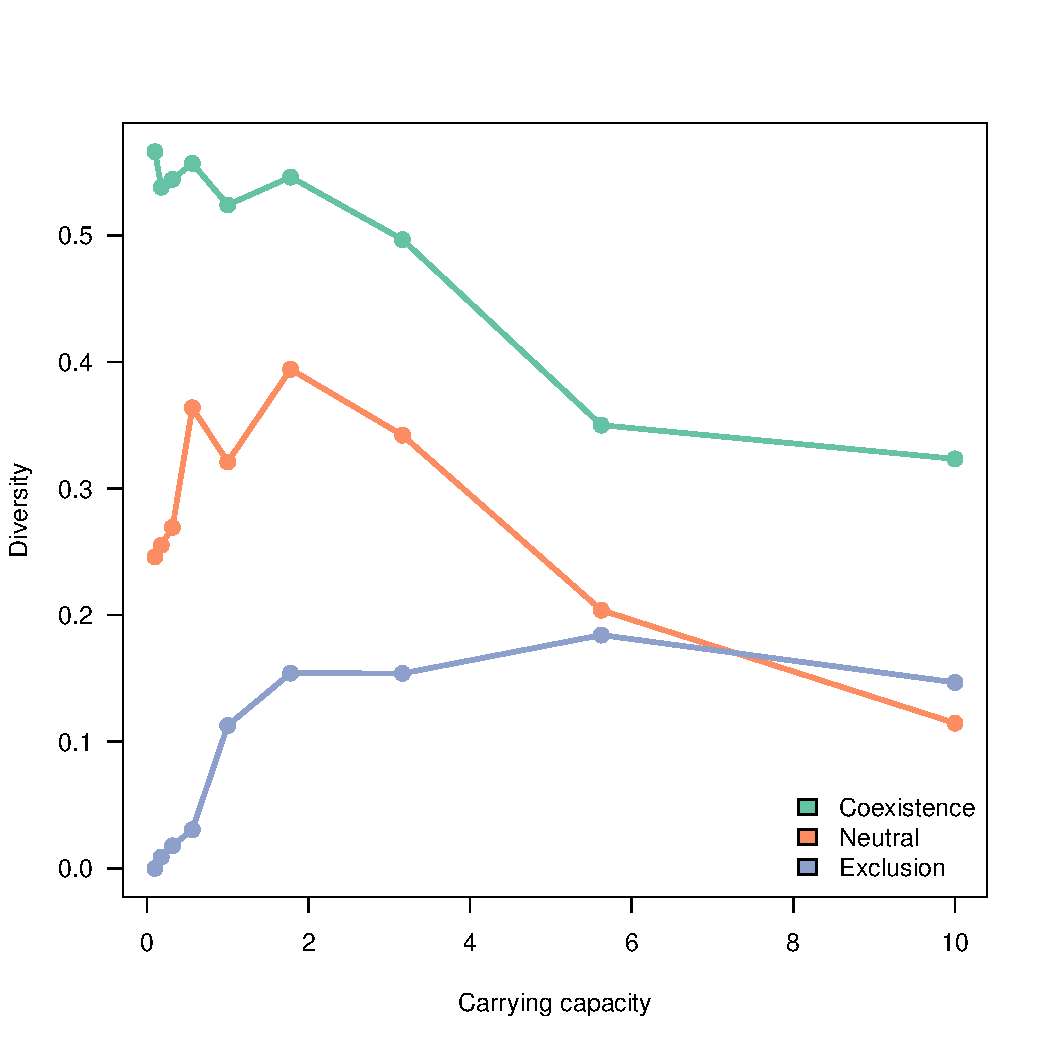
\includegraphics[width=\columnwidth]{figures/carryingcapacity.pdf}
    \caption[Effect of varying the carrying capacity.]{Effect of increasing the carrying capacity of the resource for different levels of competition ($\alpha \in \left[0.9, 1.1\right]$). For conditions of neutral coexistence or coexistence ($\alpha \leq 1$), diversity is stable until $K \approx 5$. For conditions of competition exclusion ($\alpha > 1$), diversity increases for $K < 5$, and decreases after.}
    \label{carrying}
\end{figure}

We run the simulations with the default parameters (given in
\texttt{?model\_parameters}, and in the manual). Each simulation
consists of the following code:

\begin{Shaded}
\begin{Highlighting}[]
\CommentTok{# We generate a random food web}
\NormalTok{A = nichemodel(}\FloatTok{20}\NormalTok{, }\FloatTok{0.15}\NormalTok{)}

\CommentTok{# This loop will keep on trying food webs}
\CommentTok{# until one with a connectance close enough}
\CommentTok{# to 0.15 is found}
\KeywordTok{while} \NormalTok{abs(BioEnergeticFoodWebs.connectance(A)-}\FloatTok{0.15}\NormalTok{)>}\FloatTok{0.01}
    \NormalTok{A = nichemodel(}\FloatTok{20}\NormalTok{, }\FloatTok{0.15}\NormalTok{)}
\KeywordTok{end}

\CommentTok{# Prepare the simulation parameters}
\KeywordTok{for} \NormalTok{α }\KeywordTok{in} \NormalTok{linspace(}\FloatTok{0.92}\NormalTok{, }\FloatTok{1.08}\NormalTok{, }\FloatTok{3}\NormalTok{)}
  \KeywordTok{for} \NormalTok{K }\KeywordTok{in} \NormalTok{logspace(-}\FloatTok{1}\NormalTok{, }\FloatTok{1}\NormalTok{, }\FloatTok{9}\NormalTok{)}
    \NormalTok{p = model_parameters(A, α=α,}
        \NormalTok{K=K,}
        \NormalTok{productivity=:competitive)}
    \CommentTok{# We start each simulation with}
    \CommentTok{# random biomasses in ]0;1[}
    \NormalTok{bm = rand(size(A, }\FloatTok{1}\NormalTok{))}
    \CommentTok{# And finally, we simulate.}
    \NormalTok{out = simulate(p, bm, start=}\FloatTok{0}\NormalTok{,}
          \NormalTok{stop=}\FloatTok{2000}\NormalTok{, use=:ode45)}
    \CommentTok{# And measure the output}
    \NormalTok{diversity = foodweb_evenness(out,}
                    \NormalTok{last=}\FloatTok{1000}\NormalTok{,}
                    \NormalTok{threshold=eps())}
  \KeywordTok{end}
\KeywordTok{end}
\end{Highlighting}
\end{Shaded}

The results are presented in \autoref{carrying}.

\subsection{Effect of consumer-resource body-mass ratio on
stability}\label{effect-of-consumer-resource-body-mass-ratio-on-stability}

In \autoref{vertebrate}, we illustrate how the effect of body-mass ratio
differs between food webs with invertebrates and ectotherm vertebrate
consumers.

\begin{figure}[bt]
    \centering
    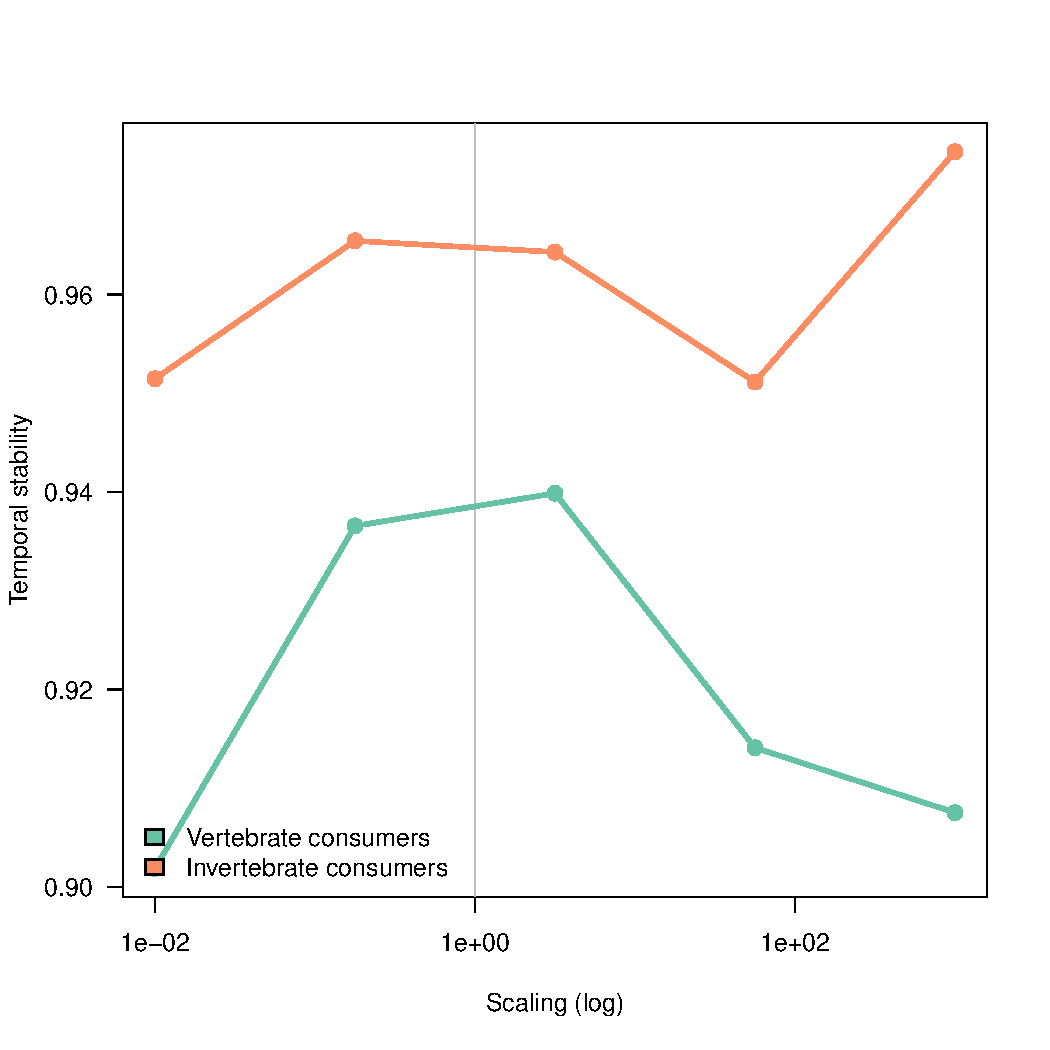
\includegraphics[width=\columnwidth]{figures/vertebrate.pdf}
    \caption[Stability as a function of organism type and allometric scaling.]{The peak of stability, in terms of allometric scaling, differs between vetebrates and invertebrates. Note that the \emph{y} axis is reversed, since more negative values indicate less variation, and therefore more temporal stability. The shaded area represents negative scaling, \emph{i.e.} predators are smaller than their preys.}
    \label{vertebrate}
\end{figure}

The body-mass ratio is controlled by the parameter \(Z\) (field
\texttt{Z} in the code), and can be changed in the following way:

\begin{Shaded}
\begin{Highlighting}[]
\NormalTok{scaling = logspace(-}\FloatTok{2}\NormalTok{, }\FloatTok{4}\NormalTok{, }\FloatTok{19}\NormalTok{) }\CommentTok{#creates an array with 19 body-mass ratio values}
\CommentTok{# Prepare the simulation parameters}
\NormalTok{p = model_parameters(A, Z=scaling[i]) }\CommentTok{#where i is a number from 1 to 19}
\end{Highlighting}
\end{Shaded}

Which species is an ectotherm vertebrate is controlled by the parameter
\texttt{vertebrate} of \texttt{model\_parameters}, which is an array of
boolean (true/false) values. In order to have all consumers be ectotherm
vertebrates, we use

\begin{Shaded}
\begin{Highlighting}[]
\NormalTok{vert = round(}\DataTypeTok{Bool}\NormalTok{,trophic_rank(A).>}\FloatTok{1.0}\NormalTok{)}
\end{Highlighting}
\end{Shaded}

so that for each network, we prepare the simulations with

\begin{Shaded}
\begin{Highlighting}[]
\CommentTok{# Prepare the simulation parameters}
\NormalTok{p = model_parameters(A,}
      \NormalTok{Z=scaling[i],}
      \NormalTok{vertebrates=vert)}
\CommentTok{# where i is a number from 1 to 19, as there are 19 body-mass ratio values in the}
\CommentTok{# scaling array}
\end{Highlighting}
\end{Shaded}

\subsection{Effect of connectance on
coexistence}\label{effect-of-connectance-on-coexistence}

We investigate the effect of connectance on species coexistence under
different scenarios of inter-specific competition rates between
producers (\autoref{connectance}). These simulations therefore measure
how the persistence of the entire food web is affected by competition at
the most basal trophic level. The persistence is used here as the
measure of coexistence.

\begin{figure}[bt]
    \centering
    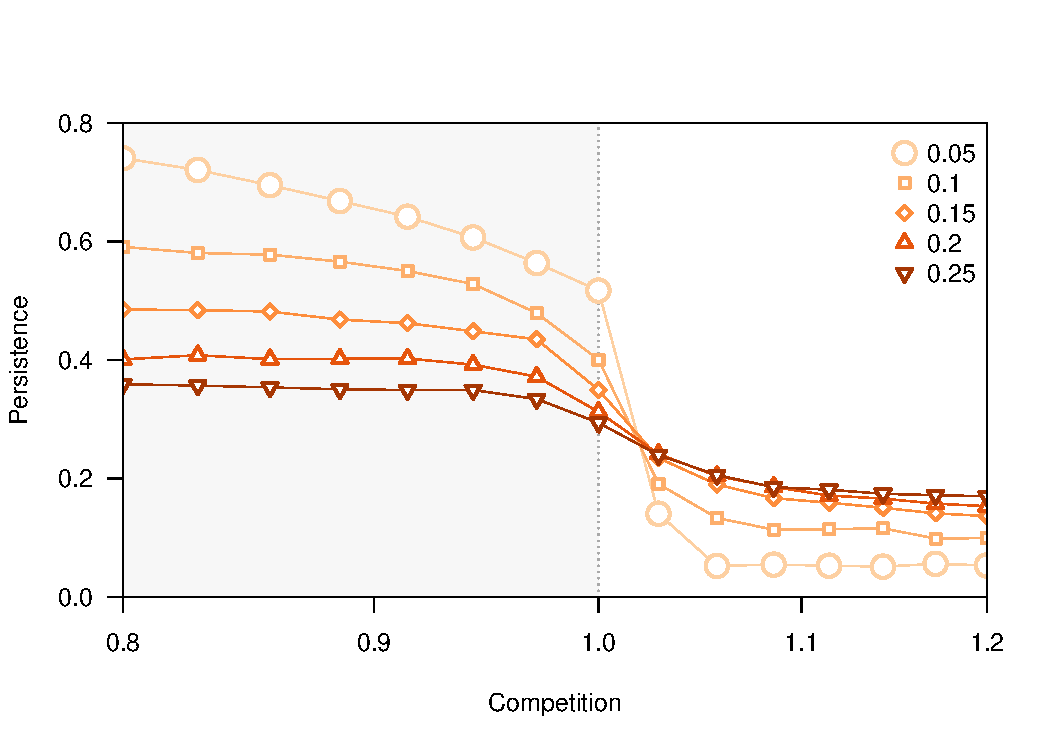
\includegraphics[width=\columnwidth]{figures/connectance.pdf}
    \caption[Connectance and competition affect species persistence.]{Although maximal species persistence is reached for values of inter-specific competition lower than unity, the increased trophic control at higher connectances allow coexistence even under stronger competition. The shaded area represents values of $\alpha$ smaller than unity, \emph{i.e.} coexistence is favored.}
    \label{connectance}
\end{figure}

\begin{Shaded}
\begin{Highlighting}[]
\KeywordTok{for} \NormalTok{co }\KeywordTok{in} \NormalTok{vec([}\FloatTok{0.05} \FloatTok{0.15} \FloatTok{0.25}\NormalTok{])}
  \CommentTok{# We generate a random food web}
  \NormalTok{A = nichemodel(}\FloatTok{20}\NormalTok{, co)}
  \KeywordTok{while} \NormalTok{abs(BioEnergeticFoodWebs.connectance(A)-co)>}\FloatTok{0.01}
      \NormalTok{A = nichemodel(}\FloatTok{20}\NormalTok{, co)}
  \KeywordTok{end}
  \CommentTok{# Prepare the simulation parameters}
  \KeywordTok{for} \NormalTok{α }\KeywordTok{in} \NormalTok{linspace(}\FloatTok{0.8}\NormalTok{, }\FloatTok{1.2} \NormalTok{, }\FloatTok{7}\NormalTok{)}
    \NormalTok{p = model_parameters(A, α=α,}
    \NormalTok{productivity=:competitive)}
    \NormalTok{bm = rand(size(A, }\FloatTok{1}\NormalTok{))}
    \CommentTok{# And finally, we simulate.}
    \NormalTok{out = simulate(p, bm, start=}\FloatTok{0}\NormalTok{,}
          \NormalTok{stop=}\FloatTok{2000}\NormalTok{, use=:ode45)}
    \CommentTok{# And measure the output}
    \NormalTok{persistence = species_persistence(out,}
                  \NormalTok{last=}\FloatTok{1000}\NormalTok{,}
                  \NormalTok{threshold=eps())}
  \KeywordTok{end}
\KeywordTok{end}
\end{Highlighting}
\end{Shaded}

Values of \(\alpha\) larger than 0 should result in competitive
exclusion in the absence of trophic interactions (Williams 2008).
Indeed, this is the case when \(Co =  0.05\) (only a single consumer
remains). Increasing connectance results in more species persisting.

\section{Conclusion}\label{conclusion}

We have presented \texttt{BioEnergeticFoodWebs}, a reference
implementation of the bio-energetic model applied to food webs. We
provided examples that can serve as templates to perform novel
simulation studies or use this model as an effective teaching tool.
Because the output can be exported in a language-neutral format (JSON),
the results obtained with this model can be analayzed in other languages
that are currently popular with ecologists, such as \texttt{R},
\texttt{python}, or \texttt{MatLab}. Because we provide a general
implementation that covers some of the modications made to this model
over the years, there is a decreased need for individual scientists to
start their own implementation, which is a both a time consuming and
potentially risky endeavor.

\textbf{Contribution statement} Authors ED and TP contributed most of
the code, which is based on apreliminary C version by DG, and was
modified during discussions with UB and DBS.

\textbf{Acknowledgements} TP acknowledges financial support from NSERC,
and an equipment grant from FRQNT. We thank the developers and
maintainers of \texttt{ODE.jl}.

\textbf{Data availability:} No data were used in this manuscript.

\textbf{Supplementary materials:}

\emph{S1} - Table of previous uses of the model, with research questions
and modifications apported.

\emph{S2} - Scripts used to generate the figures in the paper.

\section*{References}\label{references}
\addcontentsline{toc}{section}{References}

\hypertarget{refs}{}
\hypertarget{ref-baca11lvp}{}
\textbf{Bacaër}. (2011). Lotka, Volterra and the predator--prey system
(1920--1926). \emph{A Short History of Mathematical Population
Dynamics.} Springer Science + Business Media; pp. 71--6.

\hypertarget{ref-bedd75mip}{}
\textbf{Beddington}. (1975). Mutual Interference Between Parasites or
Predators and its Effect on Searching Efficiency. \emph{The Journal of
Animal Ecology.} 44:331.

\hypertarget{ref-berl04isf}{}
\textbf{Berlow et al.} (2004). Interaction strengths in food webs:
issues and opportunities. \emph{Journal of Animal Ecology.} 73:585--98.

\hypertarget{ref-bros06cbr}{}
\textbf{Brose et al.} (2006a). CONSUMER--RESOURCE BODY-SIZE
RELATIONSHIPS IN NATURAL FOOD WEBS. \emph{Ecology.} 87:2411--7.

\hypertarget{ref-bros06ase}{}
\textbf{Brose et al.} (2006b). Allometric scaling enhances stability in
complex food webs. \emph{Ecology Letters.} 9:1228--36.

\hypertarget{ref-brow04mte}{}
\textbf{Brown et al.} (2004). TOWARD A METABOLIC THEORY OF ECOLOGY.
\emph{Ecology.} 85:1771--89.

\hypertarget{ref-ches08ipc}{}
\textbf{Chesson \& Kuang}. (2008). The interaction between predation and
competition. \emph{Nature.} 456:235--8.

\hypertarget{ref-dean75mti}{}
\textbf{DeAngelis et al.} (1975). A Model for Tropic Interaction.
\emph{Ecology.} 56:881--92.

\hypertarget{ref-hatt15ppl}{}
\textbf{Hatton et al.} (2015). The predator-prey power law: Biomass
scaling across terrestrial and aquatic biomes. \emph{Science.}
349:aac6284--4.

\hypertarget{ref-kond03far}{}
\textbf{Kondoh}. (2003). Foraging Adaptation and the Relationship
Between Food-Web Complexity and Stability. \emph{Science.} 299:1388--91.

\hypertarget{ref-mcca98wti}{}
\textbf{McCann et al.} (1998). Weak trophic interactions and the balance
of nature. \emph{Nature.} 395:794--8.

\hypertarget{ref-otto07add}{}
\textbf{Otto et al.} (2007). Allometric degree distributions facilitate
food-web stability. \emph{Nature.} 450:1226--9.

\hypertarget{ref-pric12tmt}{}
\textbf{Price et al.} (2012). Testing the metabolic theory of ecology.
\emph{Ecology Letters.} 15:1465--74.

\hypertarget{ref-real77kfr}{}
\textbf{Real}. (1977). The Kinetics of Functional Response. \emph{The
American Naturalist.} 111:289--300.

\hypertarget{ref-sava04ebs}{}
\textbf{Savage et al.} (2004). Effects of Body Size and Temperature on
Population Growth. \emph{The American Naturalist.} 163:429--41.

\hypertarget{ref-tilm96bpv}{}
\textbf{Tilman}. (1995). Biodiversity: Population Versus Ecosystem
Stability. \emph{Ecology.} 77:350--63.

\hypertarget{ref-will08end}{}
\textbf{Williams}. (2008). Effects of network and dynamical model
structure on species persistence in large model food webs.
\emph{Theoretical Ecology.} 1:141--51.

\hypertarget{ref-will00sry}{}
\textbf{Williams \& Martinez}. (2000). Simple rules yield complex food
webs. \emph{Nature.} 404:180--3.

\hypertarget{ref-will07hyi}{}
\textbf{Williams et al.} (2006). Homage to Yodzis and Innes 1992:
Scaling up Feeding-Based Population Dynamics to Complex Ecological
Networks. \emph{From Energetics to Ecosystems: The Dynamics and
Structure of Ecological Systems.} Springer Science + Business Media; pp.
37--51.

\hypertarget{ref-yodz92bsc}{}
\textbf{Yodzis \& Innes}. (1992). Body Size and Consumer-Resource
Dynamics. \emph{The American Naturalist.} 139:1151--75.

\end{document}
